\documentclass[a4paper]{article}
%\documentclass[a5paper]{article}
\usepackage{microtype}
\usepackage[T1]{fontenc}
\usepackage[utf8x]{inputenc}
\usepackage{mathtools}
\usepackage{amssymb}
\usepackage{amsthm}
\usepackage{mathpple}
\usepackage{eulervm}
\usepackage{framed}
\usepackage{footnote}
\usepackage{booktabs}
\usepackage{xcolor}
\usepackage{caption}
\usepackage{subcaption}
\usepackage{braket}
%\usepackage[papersize={4.5in,6in},margin=0.5cm]{geometry} %per e-reader

\mathtoolsset{showonlyrefs}
% Colori
\definecolor{dgreen}{RGB}{0,150,0}
\definecolor{dred}{RGB}{150,0,0}

% Operatori
% --------------------
\DeclareMathOperator{\Tr}{Tr}
%\DeclareMathOperator{\det}{det}
\DeclareMathOperator{\atanh}{atanh}

% Abbreviazioni comode
% --------------------
\newcommand{\p}{\partial}
\newcommand{\abs}[1]{\lvert #1 \rvert}
\newcommand{\Real}{\mathbb{R}}
\newcommand{\Hil}{\mathcal{H}}
\newcommand{\op}[1]{\mathbf{#1}}
\newcommand{\acron}[1]{\textsc{#1}}
\newcommand{\HVT}{\acron{hvt}}
\newcommand{\QM}{\acron{qm}}
\newcommand{\I}{\mathbf{I}}
\newcommand{\red}[1]{\textcolor{dred}{#1}}
\newcommand{\green}[1]{\textcolor{dgreen}{#1}}
\newcommand{\sdot}{\centerdot}
\newcommand{\qE}{\mathcal{E}}
\newcommand{\adj}{\dagger}
\newcommand{\et}{\wedge}

% Ambienti
% --------
\newtheorem{theorem}{Theorem}[section]

\theoremstyle{definition}
\newtheorem{definition}{Definition}[section]

\let\oldproof\proof
\let\oldendproof\endproof
\renewenvironment{proof}
    {
        \begin{framed} 
        \oldproof
    }
    {
        \oldendproof 
        \end{framed}
    }

\begin{document}
\title{Notes on Contextuality}
\author{Davide Poderini}
\date{}
\maketitle

\section{Introduction}
To do.
\section{Fundamentals}
\subsection{Compatibility}
Suppose we can perform on a system a measurements of some observables $A, B, C, \ldots$,
whose outcomes will be designated by $a, b, c, \ldots$, and suppose that not all of these
observables can be measured together without disturbance.
This means that if two observables $A$ and $B$ are measured together, the result of the
measurement of $A$, can be different when it is measured before or after $B$.
If instead two observables consistently give the same results when measured
together, they are called \emph{compatible}.

More formally, consider two observables $A$ and $B$, and call\\
$S_{AB}=\{A,B,AA,AB,BA,BB,AAA,AAB,ABA,\ldots\}$ the set of all their possible
sequences of measurement. 
Then for every sequence $s \in S_{AB}$, let's denote with $a_i^s,b_i^s$ the
results of the measures of $A,B$ when they are in the $i$th position of the
sequence $s$. 
\begin{definition}[Compatibility]
    Two observable $A$ and $B$ are \emph{compatible} if we have $a_i^s=a_j^r$
    and $b_i^s=b_j^r$ for all $s,r \in S_{AB}$ and for every position $i$ in $s$
    and $j$ in $r$.
    \label{def:compatibility1}
\end{definition}

Unfortunately the definition \ref{def:compatibility1} is not experimentally testable:
we can surely test if the values of $a_i^s$ and $b_i^s$ are the same for every
$i$ in one sequence, but we can't say anything for different sequences.
A weaker, but testable, definition is the following:
\begin{definition}
    Two observable $A$ and $B$ are called \emph{compatible} if these two conditions are
    satisfied:
    \begin{enumerate}
        \item For every $s \in S_{AB}$ we have $a_i^s=a_j^s$ and $b_i^s=b_j^s$
            for every position $i,j$ of $s$.
        \item For a given state preparation, the average values
            $\langle{a_i}\rangle_s$ and $\langle{b_i}\rangle_s$ are the same for
            all $s \in S_{AB}$ and for all positions $i$ of $s$.
    \end{enumerate}
    \label{def:compatibility2}
\end{definition}

\subsection{Contextuality}
We call the \emph{context} of a measurement of an observable $A$ the set of \emph{compatible}
observables that are measured together with it.
A theory is said to be \emph{non contextual} if the predicted outcome $a$ of some observable
$A$ does not depend on the context.
If it does, we say that the theory is \emph{contextual}.

In quantum theory compatible measurements are represented by commuting operators
on a Hilbert space $\Hil$.
Without loss of generality, we can limit ourselves to consider only dichotomic
measurements, which can be represented by projectors in \QM{}.
Compatible observables in this case are equivalent to orthogonal projectors.

In \QM{} contextuality is said to be \emph{not explicit}. This means that the outcome of a measure of an
observable $A_i$ may depend on the context, but the probability for that single
observable $P(A = a)$, does not.
This is also called the \emph{no-disturbance} or \emph{no-signaling} principle.

Nonetheless, as we will show in this section, a non-contextual \HVT{} (hidden
variable theory) cannot reproduce the prediction of \QM{}.

\subsection{Joint probability}
\label{sec:joint_prob}
The problem of the existence of a non-contextual \HVT{} can be better
expressed in terms of probability distributions.
To simplify the notation we call $f(a_1,\ldots,a_k) = p(A_1=a_1, \ldots,
A_k=a_k)$ the probability that the measure of $A_1,\ldots,A_k$ gives outcomes
$a_1,\ldots,a_k$.

Quantum mechanics gives us only the joint probability distribution for
\emph{compatible} observables.
So if $\{A_1, A_2\}$ are compatible observables, but $\{A_1, A_2, A_3\}$ are
not, \QM{} gives us only $f(a_1, a_2)$, without any information about an
hypothetical $f(a_1, a_2, a_3)$.

A non-contextual \HVT{} instead, the presence of a global joint probability distribution for all
observables $f(a_1, \ldots, a_n)$ is assured by the fact that every property of
the system must have a definite value, and the uncertainty is only given by our
ignorance about the initial conditions.
From that global joint distribution one should be able to derive the quantum
mechanical ones for compatible observables $f(a_1, \ldots, a_k)$, as marginals.

The possibility of the existence of a joint probability distribution depends on
the compatibility relations between the observables.
To better visualize them, we can construct a graph where every vertex represents
an observable and two vertex are connected if the corresponding observables are
compatible, some examples are shown in figure \ref{fig:jointprob_graphs}.
\begin{figure}[h]
    \begin{subfigure}{.3\textwidth}
        \center
        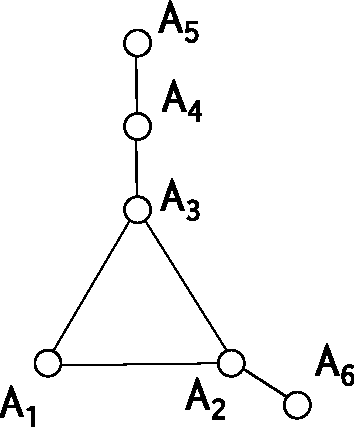
\includegraphics[width=.8\textwidth]{prob_graph1.pdf}
        \caption{}
        \label{fig:jointprob_graph1}
    \end{subfigure}
    \begin{subfigure}{.3\textwidth}
        \center
        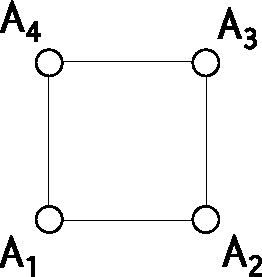
\includegraphics[width=.7\textwidth]{CHSH_obs.pdf}
        \caption{}
        \label{fig:jointprob_CHSH}
    \end{subfigure}
    \begin{subfigure}{.3\textwidth}
        \center
        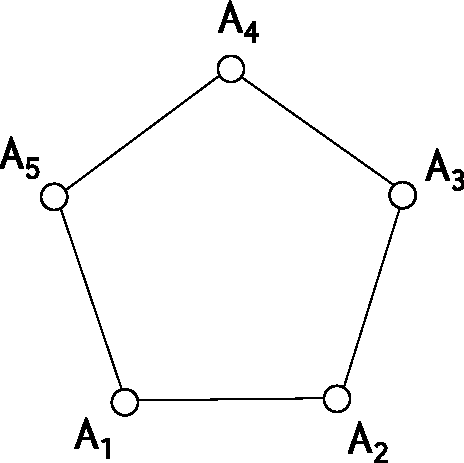
\includegraphics[width=\textwidth]{KCBS_obs.pdf}
        \caption{}
        \label{fig:jointprob_KCBS}
    \end{subfigure}
    \caption{Examples of compatibility graphs}
    \label{fig:jointprob_graphs}
\end{figure}

A sufficient condition for the existence of a joint probability
distribution is that the corresponding graph should not contain \emph{n-cycles} with $n>3$.
\footnote{The definition of \emph{n-cycle}, and other terms related to graph
theory, is given in the appendix \ref{sec:graph}.}
This statement is easily proved by constructing the joint probability for such a
graph.
\begin{proof}
If there are only 3-cycles, it is always possible to construct a global joint
probability distribution from the joint distributions of compatible observables
as follows:
first multiply together the joint distribution for every 3-cycle 
\footnote{A 3-cycle is also a clique of three mutually compatible observable, so a
joint distribution for all three variables is experimentally accessible.}
$f(a_i, a_j,a_k)$, then multiply those by the joint distributions for all the other edges,
and if an observable is present in more than one distribution divide by
$f(a_l)^{n-1}$, where $n$ is the number of terms in which it appears.
For example, for the first graph in figure \ref{fig:jointprob_graphs} we have:
\begin{equation}
    f(a_1,\ldots,a_6) = \frac{f(a_1,a_2,a_3) f(a_2, a_6) f(a_3,a_4)
    f(a_4,a_5)}{f(a_2) f(a_3) f(a_4)}
    \label{eq:jointprob_graph1}
\end{equation}
from which all the joint distributions for every edge can be obtained by summing
over the other variables.
\end{proof}
So for example it is certainly possible to construct such a distribution for
graph \ref{fig:jointprob_graph1}, but not for graphs \ref{fig:jointprob_CHSH}
and \ref{fig:jointprob_KCBS}.

While this gives no information about the existence of a joint distribution for
other graphs, the next two theorems will prove that a
similar construction is impossible in general.

\subsection{Gleason's theorem}
In the course of an analysis on the axioms of quantum theory,
Gleason proved an important theorem that poses a limit to form that the
distribution of an hypothetical \HVT{} could have.

As we said in quantum theory every yes-no test about a system can be represented by a
projector $P$ in a Hilbert space $\Hil$.
A \emph{quantum probability distribution} is a function $f(P)$ that assign to every
such projector a value such that:
\begin{align}
    &f(P) > 0 \\
    &\sum_i f(P_i) = 1 & \text{for every orthogonal base} \quad \{P_i\}
    \label{eq:gleason_th_hypotesis}
\end{align}

What Gleason proved is that every quantum probability distribution $f$ on an Hilbert space
of dimension greater than three can be written as:
\begin{equation}
    f(\op P) = \Tr(\rho P)
    \label{eq:gleason_prob}
\end{equation}
for a suitable positive semi-definite, hermitian operator $\rho$, such that
$\Tr(\rho) = 1$.
This means that the density matrix formalism is enough to describe the most general kind of
quantum probability distribution in an Hilbert space.

\begin{proof}
    To do.
\end{proof}

With this theorem is possible to deduce quantum theory from these three
postulates:
\begin{enumerate}
    \item dichotomic tests are represented by projectors in a Hilbert space.
    \item Compatible test are represented by commuting projectors.
    \item If $P$ and $Q$ are orthogonal projector then
        \begin{equation}
            \langle{P + Q}\rangle = \langle{P}\rangle + \langle{Q}\rangle
            \label{eq:QM_axiom3}
        \end{equation}
\end{enumerate}

For a non-contextual \HVT{} to exist, it has to be possible then to define a function $f(P)$ with values
$0$ or $1$ for every projector $P$ in $\Hil$.
Such a function cannot be written in the form \eqref{eq:gleason_prob}, required
by Gleason theorem for a probability distribution in $\Hil$, so for a \HVT{} we
are forced to abandon axiom (3).
%talk about axiom 3
But axiom (3) is exactly the one that guarantees the no-disturbance
principle.
If it wasn't true we could in fact choose four projectors $P,Q,R,S$ such that
\begin{equation}
    P+Q = R+S \quad \text{but} \quad 
        \langle{P}\rangle + \langle{Q}\rangle \neq
        \langle{R}\rangle + \langle{S}\rangle
\end{equation}
We can then choose another projector $T$ such that $P,Q,T$ and $R,S,T$ are
orthogonal bases, so that they represent a complete test, and it must be true that:
\begin{align}
    \langle{T}\rangle &= 1 - \langle{P}\rangle - \langle{Q}\rangle\\
    \langle{T}\rangle &= 1 - \langle{R}\rangle - \langle{S}\rangle
    \label{eq:no-dist_violation}
\end{align}
but given that $\langle{P}\rangle+\langle{Q}\rangle \neq
\langle{R}\rangle+\langle{S}\rangle$ the value of $\langle{T}\rangle$ depends on
the choice of measuring $P$ and $Q$ or $R$ and $S$, thus violating the
\emph{no-disturbance} principle.

\subsection{Kochen-Specker theorem}
\label{sec:KS_theorem}
This fundamental incompatibility is better expressed by the Kochen-Specker
theorem.

This theorem affirms that in an Hilbert space $\Hil$ of dimension $d\ge 3$, there is no
function $h$ from the set of projectors of $\Hil$ to $\{0,1\}$ such that:
\begin{equation}
    \sum_i P_i = \I \implies \sum_i h(P_i) = 1 
    \label{eq:KS_function_prop}
\end{equation}

The proofs of this theorem are usually constructive: they present a set of
projectors and show how such a function $h$ cannot be defined.
The original proof used $117$ projectors in a three dimensional space, but
smaller sets exists.
For example this proof, due to A. Peres uses only 33 rays:
%cita
\begin{proof}
    The 33 rays in question are shown in figure and listed in the table below.
    We will show that is impossible to assign value $1$ or $0$ to these rays
    without violating \eqref{eq:KS_function_prop}.
    To better visualize the argument we will use the colors \emph{green} and
    \emph{red} to represent the values $1$ and $0$ respectively.

    \begin{center}
        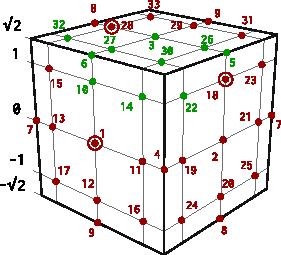
\includegraphics[scale=1.5]{KS33cube.pdf} \\
    \end{center}
    \begin{center}
    \begin{tabular}{lrlrlr}
        \multicolumn{2}{l}{Peres KS set} \\
        \toprule
        $1$ & $(1, 0, 0)$ & $12$ & $(\sqrt{2}, 0, -1)$ & $23$ & $(-1, \sqrt{2}, 1)$ \\ 
        $2$ & $(0, 1, 0)$ & $13$ & $(\sqrt{2}, -1, 0)$  & $24$ & $(1, \sqrt{2}, -1)$ \\
        $3$ & $(0, 0, 1)$ & $14$ & $(\sqrt{2}, 1, 1)$  & $25$ & $(-1, \sqrt{2}, -1)$ \\
        $4$ & $(1, 1, 0)$ & $15$ & $(\sqrt{2}, -1, 1)$  & $26$ & $(0, 1,\sqrt{2})$ \\
        $5$ & $(0, 1, 1)$ & $16$ & $(\sqrt{2}, 1, -1)$  & $27$ & $(1, 0, \sqrt{2})$ \\
        $6$ & $(1, 0, 1)$ & $17$ & $(\sqrt{2}, -1, -1)$  & $28$ & $(0, -1,\sqrt{2})$ \\
        $7$ & $(-1, 1, 0)$ & $18$ & $(0, \sqrt{2}, 1)$  & $29$ & $(-1, 0,\sqrt{2})$ \\
        $8$ & $(0, -1, 1)$ & $19$ & $(1, \sqrt{2}, 0)$  & $30$ & $(1,1,\sqrt{2})$ \\
        $9$ & $(1, 0, -1)$ & $20$ & $(0, \sqrt{2}, -1)$  & $31$ & $(-1, 1, \sqrt{2})$ \\
        $10$ & $(\sqrt{2}, 0, 1)$ & $21$ & $(-1, \sqrt{2}, 0)$  & $32$ & $(1,-1, \sqrt{2})$ \\
        $11$ & $(\sqrt{2}, 1, 0)$ & $22$ & $(1, \sqrt{2}, 1)$  & $33$ & $(-1,-1, \sqrt{2})$ \\
    \end{tabular}   
    \end{center}
    As we can see the system is symmetric under the interchange or the reversal
    of the axes $x,y,z$.
    This means that without losing generality we can paint green any of
    the rays in the orthogonal triad $\{1,2,3\}$.
    Similarly in $\{1,5,8\}$  we can choose between $5$ or $8$ (reversal of the
    $y$ axis), between $6$ or $9$ in $\{2,6,9\}$ (reversal of the $x$ axis)
     and between $31$ or $32$ in $\{4,31,32\}$ (interchange of $x$ with $y$).

    If we choose for example to paint $3,5,6$ and $32$ green, the value of the other rays
    will be fixed by the procedure shown below: \\
    \begin{center}
    \begin{tabular}{lclcl}
        $\green{3}$  & $\implies$ & \multicolumn{3}{l}{\red{$1, 2, 4, 7,11, 13, 19, 21$}}\\
        $\green{5}$  & $\implies$ & \multicolumn{3}{l}{\red{$1, 8, 15, 16$}} \\
        $\green{6}$  & $\implies$ & \multicolumn{3}{l}{\red{$2, 9, 23, 24$}} \\
        $\green{32}$ & $\implies$ & \multicolumn{3}{l}{\red{$4,12,18,31$}} \\
        \midrule
        \red{$12,2$} & $\implies$ & \green{$27$} & $\implies$ & \red{$17$} \\
        \red{$8,17$} & $\implies$ & \green{$14$} & $\implies$ & \red{$29$} \\
        \red{$29,2$} & $\implies$ & \green{$10$} & $\implies$ & \red{$33$} \\
        \red{$33,7$} & $\implies$ & \green{$30$} & $\implies$ & \red{$20$} \\
        \red{$20,1$} & $\implies$ & \green{$26$} & $\implies$ & \red{$25$} \\
        \red{$25,8$} & $\implies$ & \green{$22$} & $\implies$ & \red{$28$} \\
    \end{tabular}
    \end{center}
    
    But with this coloring the rays $\{1,18,28\}$, which form an orthogonal
    triad, are all red: we have a contradiction, and since the initial assignments where
    completely general the theorem is proved.
\end{proof}

Clearly this means that an \HVT{}, that assigns definite values $0$ or $1$ to every
yes-no test regardless of the context, is fundamentally incompatible with \QM{}.
In fact every such assignment has to satisfy \eqref{eq:KS_function_prop}, since a
set of projectors that sums to identity represent a complete test, so the
assigned values must sum to unity.
But we have just that proved that this is not possible in general for $d \ge 3$.

Other kinds of proofs exists which relies on general observables (not just
projectors), like the Peres-Mermin square described in \ref{sec:PM_square}, or
on inequalities as shown in \ref{sec:YO13}.

\subsection{Experimental Test of KS theorem}
\label{sec:exp_KS}
What we have shown is just that the \QM{} predictions are impossible to reproduce
with a classically behaving \HVT{}.
The next obvious step would be to see which way nature prefers by testing it
experimentally.
While it is possible to test the Kochen-Specker directly using the proof presented
in the last section (or other equivalent proofs), this approach is known to be
problematic.

One of the biggest problem is that every observable must be measured in more
than one, incompatible contexts. So one could not discard the possibility that
the results are influenced by the different measurement's procedure.
The inequalities, described in the next section, offer a better alternative for
experimental verification.

Another difficulty lies in the precision with which we can measure an
observable: there is always the chance that our measured observable could
differ slightly from the one we wanted to measure, this is called the \emph{finite
precision problem}.
Since it can be shown that it is possible to approximate a \acron{KS} set of rays with a
non \acron{KS} one, this is a serious problem in testing the \acron{KS}
theorem.
The way out of it is to create new versions of the \acron{KS} theorem
for imprecisely defined observables, often expressed as the already mentioned
inequalities.

The impossibility to precisely define an observable leads also to the
\emph{problem of compatibility}: we cannot assume that the observable are
compatible anymore, and as we have seen, this is a crucial assumption for
testing contextuality.
To deal with this problem, we need to add new terms to the classical bound in
inequalities, as will be described in the section \ref{sec:nc_tests}.

\section{Non-contextual inequalities}
In some systems, assuming classical
behavior implies that certain combinations of correlations between observables
are bounded by an inequality that is violated \QM{}.
This suggests another way to prove and to test the fundamental
incompatibility between \QM{} and non-contextual theories.

The most famous of these inequality is certainly the \emph{Bell theorem}, which
showed how \QM{} cannot be described by a local \HVT{}.  Since non-locality is a
particular form of contextuality, the same inequality can be used to settle the
question of the existence of non-contextual \HVT{}, and is described in section
\ref{sec:CHSH} (in the form of the \acron{CHSH} inequality).
%Scrivi nell'introduzione

Anyway, in the more general setting of contextuality we don't necessarily need two
subsystems or entanglement, as we showed in the KS theorem, a spin-1 system is enough.

It is useful to divide non-contextual inequalities into two classes:
\begin{itemize}
    \item \emph{State-dependent}, where the inequality is violated only when the
        system is in some particular state.
    \item \emph{State-independent}, where the inequality is always violated
        regardless of the state of the system.
\end{itemize}
Usually state-dependent tests involve less measurements, but obviously need a
fixed initial state, while state-independent does not.

As in section \ref{sec:joint_prob}, we can associate a graph to every
non-contextual inequality.
There are two ways to construct a graph for an inequality test: 
\begin{itemize}
    \item The \emph{Compatibility graph} is the graph constructed from the set of observables: in such a
        graph every observable is represented by a vertex and two vertex are
        connected if the corresponding observables are compatible.
    \item The \emph{Exclusivity graph} constructed from the single dichotomic exclusive events,
        where every vertex represent a yes-no measurement (a projector in the
        quantum formalism), and edges represent exclusivity (orthogonality in
        \QM{}).
\end{itemize}

In the next sections we will describe some of the most common non-contextual
inequalities.

\subsection{CHSH}
\label{sec:CHSH}
This inequality was first devised by Clauser, Horne, Shimony and Holt as an
alternative to the Bell inequality to test non-locality.
For this reason the system is composed by two 2-dimensional subsystems
(normally spin-$\frac{1}{2}$ particles) in
entanglement, that can be separated by a space-like distance.

The experimenters can measure the spin on their particles in two different directions.
The chosen observable are:
\begin{align}
    X &= \sigma_x \otimes \I &
        Z &= \sigma_z \otimes \I \\
    A &=  - \I \otimes \frac{\sigma_z + \sigma_x}{\sqrt{2}} 
        & B &=  \I \otimes \frac{\sigma_z - \sigma_x}{\sqrt{2}} 
    \label{eq:CHSH_obs}
\end{align}
and the corresponding compatibility graph is shown in figure
\ref{fig:CHSH_obs_graph}.

Since the observables measured can takes only $\pm 1$ values if we suppose a classical,
non-contextual(or local) behavior we expect:
\begin{equation}
    \langle{(X + Z) A + (Z - X) B}\rangle = 
    \langle{XA + ZA + ZB - XB}\rangle \le 2
    \label{eq:CHSH_HVT}
\end{equation}

But if, say, we prepare the system in the entangled state
\begin{equation}
    \Ket{\psi} = \frac{\Ket{0}\otimes\Ket{1} -
    \Ket{1}\otimes\Ket{0}}{\sqrt{2}} 
    \label{eq:bell_state_psim}
\end{equation}
\QM{} predicts:
\begin{equation}
    \langle{XA}\rangle + \langle{ZA}\rangle + \langle{ZB}\rangle
    - \langle{XB}\rangle = 2\sqrt{2}
    \label{eq:CHSH_QM}
\end{equation}
so \eqref{eq:CHSH_HVT} is violated by quantum mechanics.
Notice that for the inequality to be violated the system has to be in a particular entangled
state, so this is an example of a state-dependent inequality.

We can also write \eqref{eq:CHSH_HVT} using directly probabilities for exclusive events:
\begin{multline}
    p(11| X A) + p(-1-1| X A) +
    p(11| Z B) + p(-1-1| Z B) +\\
    p(11| Z A) + p(-1-1| Z A) +
    p(-11| X B) + p(1-1| X B) \le 3
\end{multline}
where $p(ab|AB)$ represents the probability of having oucomes $a$ and $b$
measuring the properties $A$ and $B$.
The events involved are represented in the exclusivity graph \ref{fig:CHSH_proj_graph}.

It can be shown that in \QM{} the maximum value of this sum is $2+\sqrt{2}$, so
the inequality is again violated.
\begin{figure}[h]
    \begin{subfigure}{.3\textwidth}
        \centering
        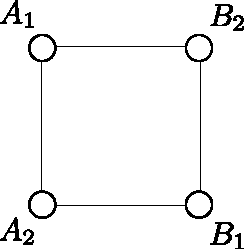
\includegraphics[width=\textwidth]{CHSHog.pdf}
        \caption{Compatibility graph}
    \label{fig:CHSH_obs_graph}
    \end{subfigure}
    \begin{subfigure}{.7\textwidth}
        \centering
        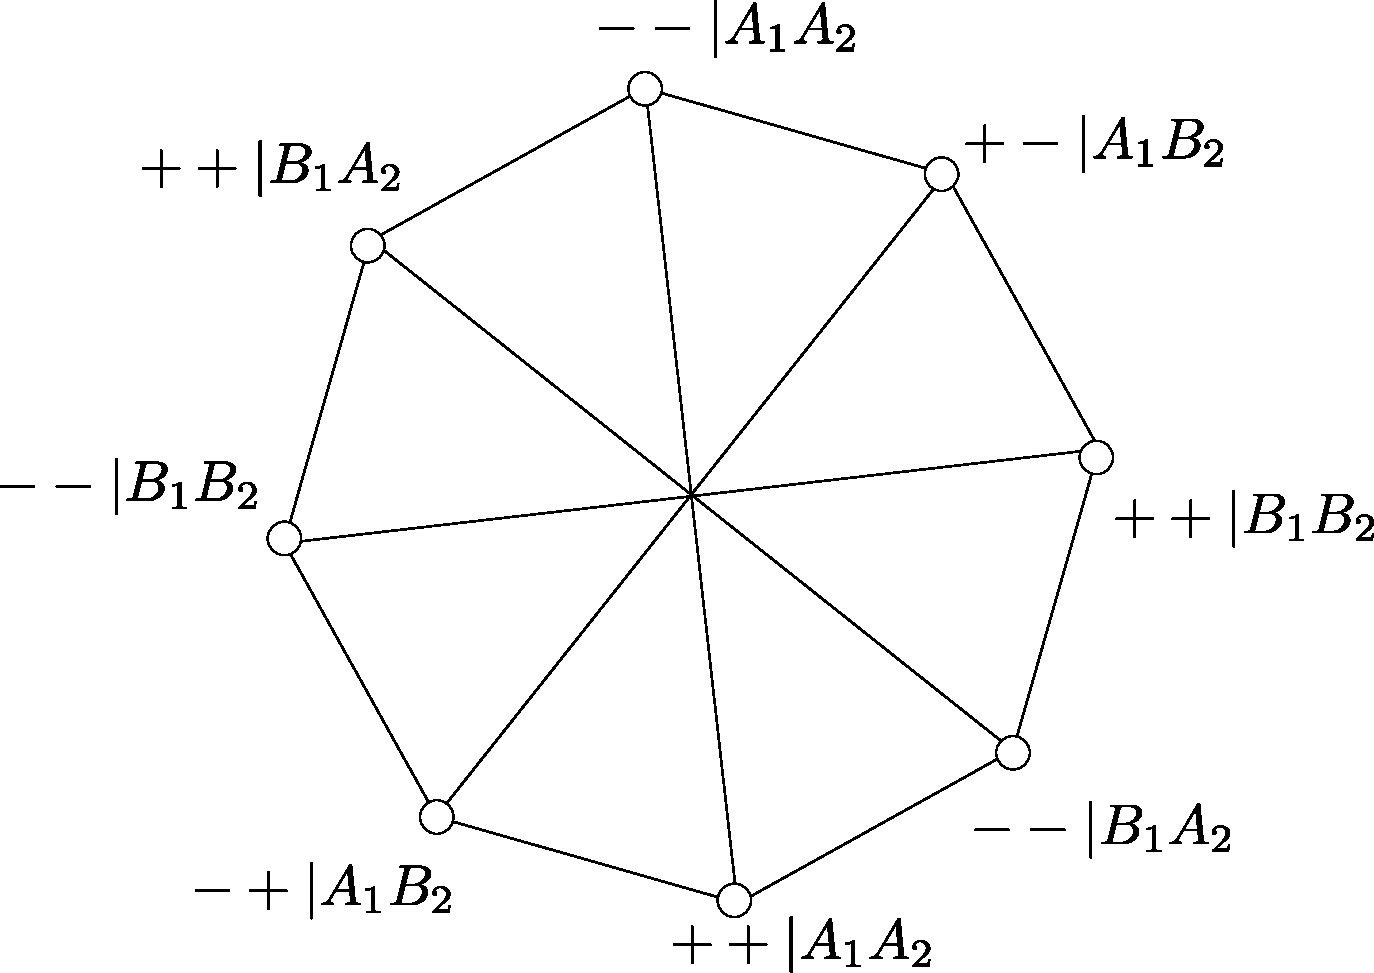
\includegraphics[width=\textwidth]{CHSHpg.pdf}
        \caption{Exclusivity graph}
    \label{fig:CHSH_proj_graph}
    \end{subfigure}
    \caption{Graphs for the \acron{CHSH} inequality}
    \label{fig:CHSH_graphs}
\end{figure}
\subsection{KCBS}
A more recent example of a state-dependent non-contextual inequality is
called the \acron{KCBS} inequality, from Klyachko, Can, Binicioglu and Shumovsky.

Here we have five dichotomic observables which can take values $\{0,1\}$ that satisfy the
exclusivity relations shown in figure \ref{fig:KCBS_graph}.
\begin{figure}[h]
        \centering
        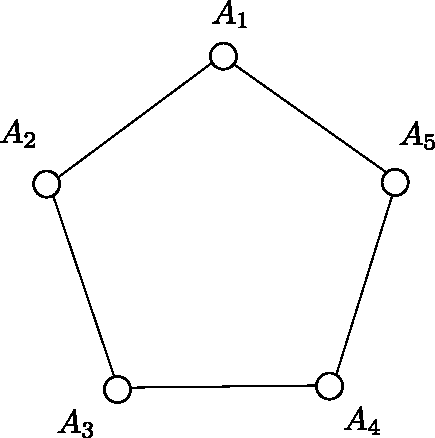
\includegraphics[width=0.4\textwidth]{KCBSog.pdf}
        \caption{Exclusivity graph for the \emph{KCBS} inequality}
    \label{fig:KCBS_graph}
\end{figure}

Classically, since only 2 observables can be assigned the value
$1$ to satisfy the exclusivity graph, we have the inequality.
\begin{equation}
    \sum_{i=1}^5 a_i \le 2
    \label{eq:KCBS_HVT_1}
\end{equation}

This inequality is often presented in another form, using the
observables $B_i = 2 A_i - 1$ instead that takes the values $\{1,-1\}$, so that
\eqref{eq:KCBS_HVT_1} becomes:
\begin{equation}
    \langle{B_1B_2}\rangle + 
    \langle{B_2B_3}\rangle + 
    \langle{B_3B_4}\rangle + 
    \langle{B_4B_5}\rangle + 
    \langle{B_5B_1}\rangle \ge - 3 
    \label{eq:KCBS_HVT_2}
\end{equation}

In \QM{} the $A_i = \Ket{a_i}\Bra{a_i}$ are projectors in a 3-dimensional
Hilbert space, with orthogonality relations given by the graph
\ref{fig:KCBS_graph}.
The inequality \eqref{eq:KCBS_HVT_2} can be implemented measuring $B_i = 1 -
S_i^2$, where the $S_i$ are the spin observables for a spin-1 particle in five
different direction.
For example we can use the rays:
\begin{align}
    \Ket{a_1} &= \left(1,0,\sqrt{\cos(\pi/5)}\right) \\
    \Ket{a_2} &= \left(-\cos(\pi/5),\sin(\pi/5),\sqrt{\cos(\pi/5)}\right)\\ 
    \Ket{a_3} &=\left(-\cos(\pi/5),-\sin(\pi/5),\sqrt{\cos(\pi/5)}\right)\\
    \Ket{a_4} &= \left(-\cos(2\pi/5),\sin(2\pi/5),\sqrt{\cos(\pi/5)}\right)\\
    \Ket{a_4} &=\left(-\cos(2\pi/5),-\sin(2\pi/5),\sqrt{\cos(\pi/5)}\right)\\
    \label{eq:KCBS_rays}
\end{align}
directed along the vertices of a pentagram as in figure \ref{fig:KCBS_pent}.
\begin{figure}[h]
    \centering
    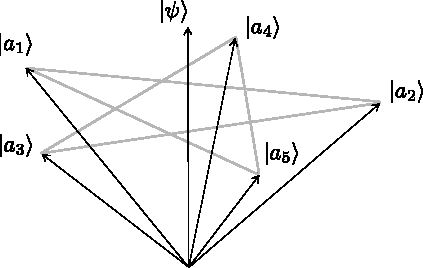
\includegraphics[width=.7\textwidth]{KCBS_pent.pdf}
    \caption{Rays corresponding to the projectors $A_1,\ldots,A_5$ }
    \label{fig:KCBS_pent}
\end{figure}
If we measure them on the state $\Ket{\psi} = (1,0,0)$ we have
\begin{equation}
    \sum_{i=1}^5 \left|\Braket{a_i|\psi}\right|^2 = \sqrt{5} > 2
    \label{eq:KCBS_QM_1}
\end{equation}
which correspond to a violation of $5-4\sqrt{5}$ for the inequality
\eqref{eq:KCBS_HVT_2}.
\subsection{Peres-Mermin square}
\label{sec:PM_square}
This state-independent inequality has its origin in another proof of the
Kochen-Specker theorem.

Suppose to have a system similar to the one used for the \acron{CHSH}
inequality: two particles of spin-$\frac{1}{2}$, and consider the
observables:
\begin{align}
    A_{11}&=\I\otimes\sigma_z  &A_{12}&=\sigma_z\otimes\I &A_{13}&=\sigma_z\otimes\sigma_z \\
    A_{21}&=\sigma_x\otimes\I  &A_{22}&=\I\otimes\sigma_x &A_{23}&=\sigma_x\otimes\sigma_x \\
    A_{31}&=\sigma_x\otimes\sigma_z  &A_{32}&=\sigma_z\otimes\sigma_x &A_{33}&=\sigma_y\otimes\sigma_y \\
    \label{eq:PM_square}
\end{align}
The last element of every row is the product of the other two, and the same
is true for the columns, except for the last one since: 
\begin{equation}
    (\sigma_z\otimes\sigma_z) (\sigma_x\otimes\sigma_x) = - \sigma_y\otimes\sigma_y
    \label{eq:PM_lastcol}
\end{equation}

For this reason a fixed assignment of values $\{1,-1\}$ to every observable in
\eqref{eq:PM_square} is not possible, and this rules out the possibility of
having a non-contextual \HVT{} to explain those measures.

This can also be rephrased in the form of an inequality:
\begin{multline}
    \langle{A_{11}A_{12}A_{13}}\rangle + 
    \langle{A_{21}A_{22}A_{23}}\rangle + 
    \langle{A_{31}A_{32}A_{33}}\rangle +\\ +
    \langle{A_{11}A_{21}A_{31}}\rangle + 
    \langle{A_{12}A_{22}A_{32}}\rangle - 
    \langle{A_{13}A_{23}A_{33}}\rangle \le 4 
    \label{eq:PM_ineq}
\end{multline}
Which holds classically, since the third element in every correlation is the
product of the other two.

But in \QM{} we have:
\begin{multline}
    \langle{A_{11}A_{12}A_{13}}\rangle + 
    \langle{A_{21}A_{22}A_{23}}\rangle + 
    \langle{A_{31}A_{32}A_{33}}\rangle +\\ +
    \langle{A_{11}A_{21}A_{31}}\rangle + 
    \langle{A_{12}A_{22}A_{32}}\rangle - 
    \langle{A_{13}A_{23}A_{33}}\rangle = 6 
\end{multline}
so the inequality \eqref{eq:PM_ineq} is violated for every state of the system.

\subsection{Yu-Oh's 13 rays inequality}
\label{sec:YO13}
The proofs of the Kochen-Specker theorem we have seen are all based on the
impossibility of assigning definite value to a groups of observable.

This proof involves instead a set of 13 rays, where KS-type assignments are
possible, but every such assignment satisfy an inequality violated by \QM{}.

The rays used in the proof are:
\begin{align}
    a_1 &= (1,0,0) &a_2 &= (0,1,0) &a_3 &= (0,0,1) && \\
    b_1 &= (0,1,1) &b_2 &= (1,0,1) &b_3 &= (1,1,0) &&\\
    c_1 &= (0,1,-1) &c_2 &= (1,0,-1) &c_3 &= (1,-1,0) &&\\
    d_1 &= (-1,1,1) &d_2 &= (1,-1,1) &d_3 &= (1,1,-1) &d_4 &= (1,1,1)\\
    \label{eq:YO13_rays}
\end{align}
and they satisfy the exclusivity conditions showed in the graph in figure
\ref{fig:YO13_graph}.
\begin{figure}[h]
    \centering
    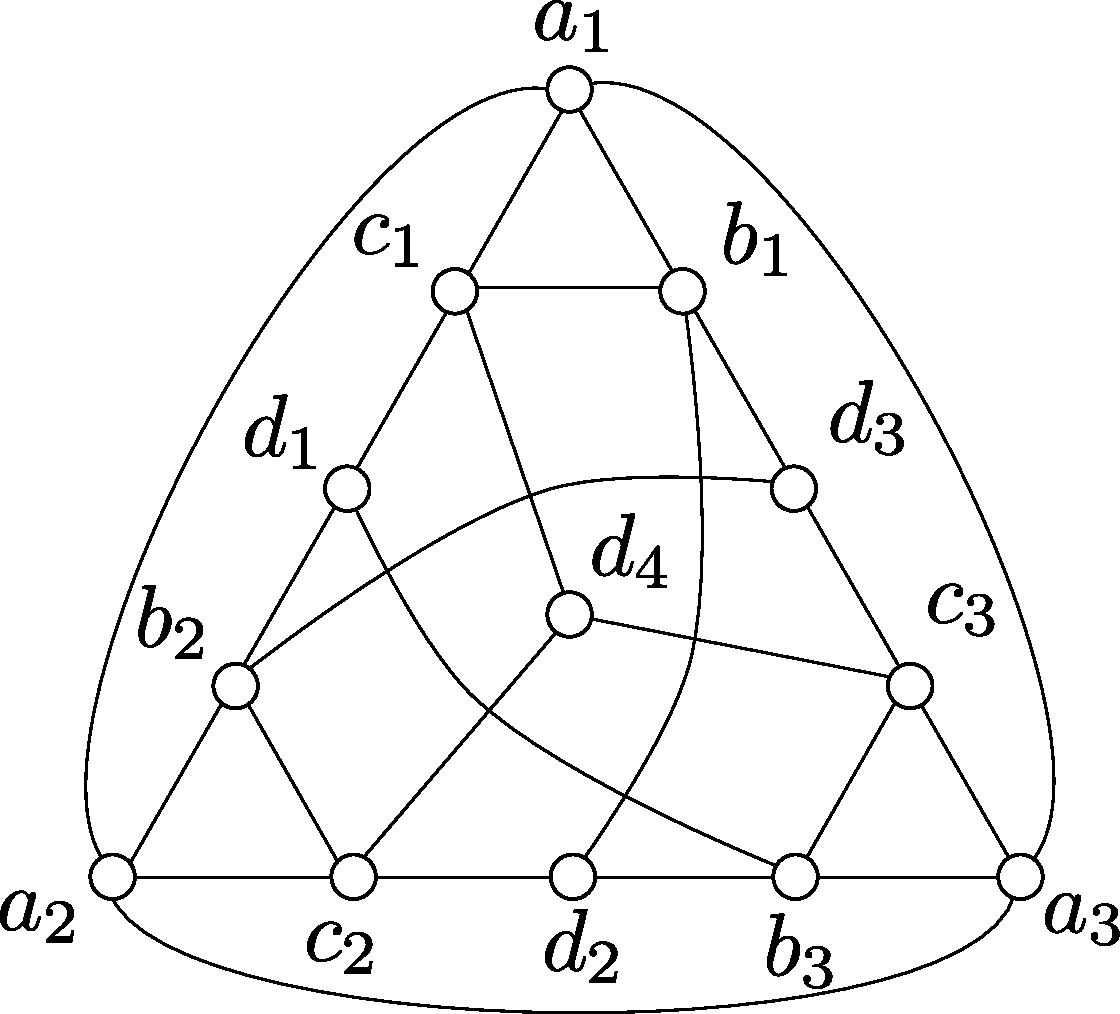
\includegraphics[width=0.6\textwidth]{YO13pg.pdf}
    \caption{Exclusivity graph for the 13 rays}
    \label{fig:YO13_graph}
\end{figure}

If we try to assign values $\{0,1\}$ to these rays we notice that only one of
the rays $d_i$ can be assigned the value $1$.

\begin{proof}
Like we did in section \ref{sec:KS_theorem}, let's use the colours green and
red instead the values $1$ and $0$ respectively.
We first show that if $d_4$ is green, none of the other $d_i$ can be green.

If for instance $d_4$ and $d_1$ are green then $b_3,c_3$ and $b_2,c_2$
must be red, which means that $a_2$ and $a_3$ have to be green but this is not
allowed. The same is true for $d_2$ and $d_3$.

Moreover only one between $d_1,d_2,d_3$ can be green at once, for example if $d_1$ and
$d_2$ were both green, then $b_1,c_1$ and $b_2,c_2$ have to be red which means
that $a_1$ and $a_2$ must be green and this is again not possible.
For symmetry reason, the same is true for $d_2,d_3$ and $d_1,d_3$, so we must
conclude that only one between $\{d_1,d_2,d_3,d_4\}$ can be green in every
assignment.
\end{proof}

From this we have that every non-contextual \HVT{} must obey the inequality
\begin{equation}
    \sum_{i=1}^4 \langle{d_i}\rangle \le 1
    \label{eq:YO13_HVT}
\end{equation}
In \QM{} instead we have:
\begin{equation}
    \sum_{i=1}^4 d_i = \frac{4}{3}\I \quad \implies \quad
    \sum_{i=1}^4 \langle{d_i}\rangle = \frac{4}{3} 
    \label{eq:YO13_QM}
\end{equation}
and no non-contextual \HVT{} can reproduce this result.

If we use the observable $A_i = 2\I - P_i$, where $P_i$ are the
projectors associated with the rays \eqref{eq:YO13_rays}, that takes the values
$\{1,-1\}$, we can write the inequality
\begin{equation}
    \sum_i \langle{A_i}\rangle - \frac{1}{4} \sum_{(i,j)} \langle{A_i A_j}\rangle \le 8
    \label{eq:YO13_HVT2}
\end{equation}
where the sum in the second term is extended only to $i,j$ connected by an edge
in the graph \ref{fig:YO13_graph}.
As it can easily be proved in \QM{} we have:
\begin{equation}
    \sum_i A_i - \frac{1}{4} \sum_{(i,j)} A_i A_j = \frac{25}{3} \I
    \label{eq:YO13_QM2}
\end{equation}
so the inequality \eqref{eq:YO13_HVT2} is violated for every state.

\subsection{Graph theoretical approach}
The \emph{exclusivity} graph is a powerful instrument to
analyze inequalities.
In fact from the graph, we can easily deduce if the inequality is
violated by \QM{}, and how much is the violation.

As we did in section \ref{sec:CHSH} for the \acron{CHSH} inequality, every
non-contextual inequality can be expressed as a positive linear combination of
probabilities:
\begin{equation}
    A = \sum_i w_i P_i
    \label{eq:prob_ncineq}
\end{equation}

To every such a linear combination we can associate an exclusivity graph as
described at the beginning of this section\footnote{The graph is
weighted if the coefficients $w_i \neq 1$, the following theorems are valid
also in this case.}, where now the dichotomic observable $A_i$ that takes
values $\{0,1\}$, is the one associated with the $i$th event, so that
$\langle{A_i}\rangle = P_i$. % spiega meglio
Once we construct this graph we can derive the inequality and its violation in
\QM{} (if present) using the following theorems.

\begin{theorem}
    Given a graph $G$ associated with a non-contextual inequality $A$, the maximum value
    attainable by a non-contextual \HVT{} is equivalent to the independence number
    $\alpha(G)$ of the graph while the maximum for quantum theory is the Lovàsz number
    $\theta(G)$ of the graph, and
    \begin{equation}
        \alpha(G) \le \theta(G)
    \end{equation}
    \label{th:nc_graph_indilov}
\end{theorem}
\begin{proof}
    In a non-contextual \HVT{}, being deterministic, each events has probability
    $0$ or $1$.
    The maximum of $A$ is attained when the value $1$ is assigned to the maximum
    possible number of events, $A$ in this case corresponds to the cardinality
    of the largest set of independent vertices, that is \emph{independence
    number} $\alpha(G)$ of the graph.

    In \QM{} every event corresponds to a unitary ray in a given Hilbert space,
    and connected vertices correspond to orthogonal rays, this is exactly an
    \emph{orthonormal representation} of the graph $G$.
    Since the probabilities are $P_i = \abs{\braket{a_i | \psi}}$ for a
    given $\Ket{\psi}$, the maximum of $A$ is clearly given by the
    \emph{Lovàsz number} of the graph $G$ as defined in
    \eqref{eq:Lovasz_theta}.

    The inequality follows directly by the Lovàsz's sandwich theorem
    \ref{th:sandwich}.
\end{proof}

Notice that $\alpha(G)$ is only an upper bound for the maximum value attainable
for a non-contextual \HVT{}, since it does not impose the condition that in every
complete test the probabilities sums to $1$.
For example for the graph in figure \ref{fig:YO13_graph} the independence number
is $\alpha(G) = 5$, but in every independent set with that number of vertices
all the $d_i$ are included (i.e. have value $1$) which as we
said is impossible, at least when is implemented in dimension $d=3$.
To avoid this we can give a different weight, $w=2$ to vertices $a_i,b_i, c_i$
so that the independence number becomes $\alpha(G) = 7$ reached with an 
independent set with one vertex in every 3-clique, and the Lovasz number
$\theta(G)= $.
%What we are looking for in that case is the cardinality $\beta_d$ of the largest
%independent set that has a vertex in every d-clique, this number is always
%$\beta_d \le \alpha(G)$, in the previous case for example is $4$.

\begin{theorem}
    The inequality associated with the graph $G$ is violated if and only if $G$
    contain as a subgraph a cycle graph $C_n$ of $n\ge5$ or its complement.
    \label{th:nc_graph_indinum}
\end{theorem}
\begin{proof}
    Indeed if the graph have got no such odd cycles or their complement then is
    perfect, by the strong perfect graph theorem \ref{th:strong_perfect_graph}.
    In this case we have
    \begin{equation}
        \alpha(G) = \omega(\bar G) = \chi(\bar G)
    \end{equation}
    so for the sandwich theorem \ref{th:sandwich}
    \begin{equation}
        \alpha(G) = \theta(G)
    \end{equation}
    and we have no violation.
\end{proof}

\section{Problems in non-contextual tests}
\label{sec:nc_tests} 

\subsection{Correction terms in inequalities}
As we already said in section \ref{sec:exp_KS} compatibility of observable
cannot be assured in an experimental test.
This and other effects have to be considered in a test of quantum contextuality.

As before, consider a system on which we can perform measurements
of dichotomic $\pm1$ observables $\{A,B,C\ldots\}$, that are not all compatible.
We want to consider the results of the disturbance that theoretically
compatible measurements have on one another.
Let's call
\begin{equation}
    P\left(A_1^{a_1} B_2^{b_2} C_3^{c_3}\cdots\right)
\end{equation}
the probability that the sequence of measurements $A_1 B_2 C_3 \cdots$ 
gives as outcomes $a_1 b_2 c_3\cdots $, where the lower indices are used to
distinguish observables in different positions of the sequence.

The probability $p_f(AB)$ of a flip in the outcome of $B$ due to the measure of $A$
then can be expressed as:
\begin{equation}
    p_f(AB) = P\left(B_1^+ \et A_1 B_2^-\right) + P\left(B_1^- \et A_1 B_2^+\right)
\end{equation}
The problem is that those probabilities are not accessible by experiment.
Instead what we can measure is the probability
\begin{equation}
    p_E (BAB) = P\left(B_1^+ A_2 B_3^-\right)+P\left(B_1^- A_2 B_3^+\right)
\end{equation}
and if we \emph{assume} that additional measurements can only increase the disturbance
of a system, we have 
\begin{equation}
    p_f(AB) \le p_E (BAB)   
    \label{eq:pe_ass1}
\end{equation}
since the probability of a flip cannot decrease with the addition of the first
measurement of $B$.
From this considerations follows that:
\begin{equation}
    P\left(A_1^a B_2^b\right) \le P(A_1^a \et B_1^b) + p_f(AB) \le P(A_1^a \et B_1^b) + p_E(BAB) 
    \label{eq:prob_noncomp}
\end{equation}

So for example the \acron{CHSH} inequality becomes:
\begin{multline}
    P(X_1^+ A_2^+) + P(X_1^- A_2^-) +
    P(Z_1^+ B_2^+) + P(Z_1^- B_2^-) +\\
    P(Z_1^+ A_2^+) + P(Z_1^- A_2^-) +
    P(X_1^- B_2^+) + P(X_1^+ B_2^-) \le \\
    \le 3 + 2 p_E(AXA) + 2p_E(BZB) +
    +2 p_E(AZA) + 2 p_E(XBX)
\end{multline}
The correlations $\langle{A_1B_2}\rangle$ instead are bounded by
\begin{equation}
    \langle{A_1B_2}\rangle - p_f(AB)\le \langle{AB}\rangle \le \langle{A_1B_2}\rangle + p_f(AB)
\end{equation}
in this case the \acron{CHSH} becomes
\begin{multline}
    \abs{\langle{X_1A_2 + Z_1A_2 + Z_1B_2 - X_1B_2}\rangle} \le 
    2 +  2p_E(AXA) +\\ 
    + 2p_E(AZA) + 2p_E(BZB) + 2p_E(BXB)
\end{multline}

\subsubsection{A more general bound for $p_f$}
Assumption \eqref{eq:pe_ass1} is not always valid.
Another, more general, approach is to measure the probability of a flip in
some set of sequences of measurements $S=\{AA, BB, BAB, ABA, BBB, BBA, AAA, AAB, BAAB,\ldots\}$, in
order to find the probability of a deviation from ideal compatibility.

For example, for sequences of three measurements in
\begin{equation}
 S_3 =\{ABA,BAB,BBA,AAB,ABB,BAA,AAA,BBB\}    
\end{equation}
we will measure the probabilities:
\begin{align}
    p_E(ABA) &= P(A_1^+ B_2 A_3^-) + P(A_1^- B_2 A_3^+) \\ 
    p_E(BAB) &= P(B_1^+ A_2 B_3^-) + P(B_1^- A_2 B_3^+) \\ 
    &\vdots\\
    p_E(BBB) &= 1 - P(B_1^+ B_2^+ B_3^+) + P(B_1^- B_2^- B_3^-)
\end{align}
and sum them, obtaining
\begin{equation}
    p_E^3(AB) = p_E(ABA) + p_E(BAB) + p_E(ABB) + p_E(BAA) + p_E(AAA) + p_E(BBB)
\end{equation}
where we excluded the terms $p_E(BBA)$ and $p_E(AAB)$ since their contribution
is already considered in $p_E(BBB)$ and $p_E(AAA)$ respectively.

We \emph{assume} now that when the observable are compatible, the
non-contextuality holds.
This will happen with probability
\begin{equation}
    p_C(AB) \ge 1 - p_E^3(AB)
\end{equation}
in those cases we cannot have a flip, so we conclude that
\begin{equation}
    p_f(AB) \le p_E^3(AB)
    \label{eq:pe_ass2}
\end{equation}
obtaining another experimentally measurable bound to the probability of a flip.

Clearly this approach is more general than the previous one, where only terms
like $p_E(BAB)$ are considered.

%\subsubsection{Extended inequality based on averages}
%Another way to measure the deviation from compatibility of two observable is by
%using directly the definition \eqref{def:compatibility2}, measuring those
%averages for a large number of state preparations.
%Let's assume that we have found that:
%\begin{equation}
%    \abs{\langle{b_1}\rangle_{BA} -
%    \langle{b_2}\rangle_{AB}} \le \varepsilon_{BA} 
%    \label{eq:comp_avg_diff}
%\end{equation}
%
%From this we have that
%\begin{equation}
%    \abs{P\left(B_1^{\pm}A_2\right) - P\left( A_1 B_2^{\mp}\right)} \le
%    \frac{\varepsilon_{BA}}{2}
%    \label{eq:comp_prob_diff}
%\end{equation}
%Now, since 

\subsection{Noise in quantum measurements}
Not only the bound in inequality, but also the value of its
violation in \QM{} is affected by lack of compatibility.

To give a more accurate description of this effect we can think of the system as
going through a noisy channel between every measurements.
Quantum mechanically this can be represented by a (non unitary) \emph{quantum
operation} $\qE(\rho)$ acting on the density matrix $\rho$ of the system, which
can be expressed in the \emph{operator sum} representation as
\begin{equation}
    \rho' = \sum_i E_i^\adj \rho E_i
    \label{eq:kraus_evolution}
\end{equation}
where $E_i$ are the \emph{Kraus operators} associated with $\qE$.
\footnote{Check Nielsen Chuang, \emph{Quantum computation and quantum
information}.}

Let's again consider two $\{+1,-1\}$ dichotomic observables $A$ and $B$.
The quantum state after the measure of $A$ will be
\begin{equation}
    \rho_A^+ = \frac{P_A^+\rho P_A^+}{\Tr\left( P_A^+\rho \right)} 
    \quad \text{or} \quad
    \rho_A^- = \frac{P_A^-\rho P_A^-}{\Tr\left( P_A^-\rho \right)}
    \label{eq:projective_measure_A}
\end{equation}
with probability $P(+|A) = \Tr\left( P_A^+ \rho \right)$ or $P(-|A) = \Tr\left(
P_A^- \rho \right)$ respectively.

Applying the noise and measuring $B$ after this first measurement we have that
the probability of having $B=\pm 1$ is
\begin{equation}
    P(+\pm|AB) = \Tr\left( P_B^\pm \qE\left(P_A^+\rho P_A^+\right) \right)
    \quad \text{or} \quad
    P(-\pm|AB) = \Tr\left( P_B^\pm \qE\left(P_A^-\rho P_A^-\right) \right)
\end{equation}
so the correlation becomes
\begin{multline}
    \langle{AB}\rangle = P(++|AB) + P(--|AB) + P(+-|AB) + P(-+|AB) =\\
    = \Tr\left( P_B^+ \qE\left(P_A^+\rho P_A^+ - P_A^-\rho P_A^-\right) +
        P_B^- \qE\left(P_A^-\rho P_A^- - P_A^+\rho P_A^+\right)
    \right)
\end{multline}
Similarly we can calculate the effect of the noise in a sequence of more
measurements. 

\subsection{Stochastic noise in non-contextual \HVT{}}
Here we want to construct a model to show how a noisy measurement process can
change the bound in non-contextual inequality.

Remember that in a hidden variable theory the state of the system is described
by a variable $\lambda$ (or by a distribution $p(\lambda)$) from which we can
deduce the value (or the joint distribution) of every measurable property $A(\lambda)$.
We can then think of the noise as a stochastic process that for every
measurement changes the state of the system $\lambda \rightarrow \lambda'$ with a certain
probability.
In general we can think of the system evolving as
\begin{equation}
    \lambda_1 \rightarrow\lambda_2 \rightarrow\cdots\rightarrow\lambda_n
    \label{eq:noiseHV_evolution}
\end{equation}
with a certain probability $p_{\lambda_1\lambda_2\ldots\lambda_n}$.

By using this model we can the averages for non perfectly compatible are given
by, for example:
\begin{align}
    \langle{AB}\rangle = \langle{a_1b_2}\rangle_{AB} &= \sum
    p_{\lambda_1\lambda_2}A(\lambda_1)B(\lambda_2)\\
    \langle{BAB}\rangle = \langle{b_1a_2b_3}\rangle_{BAB} &= \sum
    p_{\lambda_1\lambda_2\lambda_3}B(\lambda_1)A(\lambda_2)B(\lambda_3)
    \label{eq:noiseHV_avg}
\end{align}

An important point is that the evolution of the system should not be dependent
on the observable measured.
If not, we would in fact just reintroduce contextuality in our model, and we
could then easily violate every non-contextual inequality.

What we want to describe here are the inevitable deviations from ideal
compatibility of our observable. 
Although there's no reason to assume non contextuality for non compatible
observable, even in a non contextual \HVT{}, what we assume here is that the
random and (hopefully) small deviation from compatibilty can be described by an
evolution independent on the measurement context, also called a \emph{non contextual
evolution}. 

\subsubsection{Markov noise}
An interesting case is when this evolution can be described as a \emph{Markov
chain}.
This is possible if we assume that the probability of transition is the same at
every step, that is, the process has no memory.

Consider a system with $n$ states $\lambda_1,\ldots,\lambda_n$. 
To every distribution $p(\lambda)$ we can assign a \emph{probability vector} defined as
$p_i = p(\lambda_i)$.
Our markov process is then completely defined by a $n\times n$ matrix $T$, the
\emph{transition matrix}, whose elements $T_{ij}$ represent the transition
probabilities $\lambda_i \rightarrow \lambda_j$.
At every step the probability vector $p^{(n)}$ evolves as
\begin{equation}
    p_i^{(n+1)} = \sum_j T_{ij} p_j^{(n)}
    \label{eq:markov_evolution}
\end{equation}
Clearly every transition matrix must fulfill the condition $\sum_i T_{ij} = 1$.

\begin{theorem}
    For every non-contextual inequality $S$ there exists a maximum bound $S_{M}$ to the
    possible violation and this bound can always be reached by a suitable Markov process.
    \label{th:noise_max_violation}
\end{theorem}
\begin{proof}
    A non-contextual inequality is in general a sum of averages:
    $S = \langle{AB\ldots C}\rangle + \cdots$.
    If we call
    \begin{equation}
        S_{k_1 k_2 \ldots k_m} =
        A(\lambda_{k_1})B(\lambda_{k_2})\cdots C(\lambda_{k_m}) + \cdots
    \end{equation}
    and denote by
    \begin{equation}
         S_M = S_{\bar k_1 \bar k_2 \ldots \bar k_m}
        \label{eq:max_ineq_S}
    \end{equation}
    the maximum of $S_{k_1k_2\ldots k_m}$, from \eqref{eq:noiseHV_avg} we have:
    \begin{equation}
        S=
        \sum_{k_1 k_2\ldots k_m} p_{\lambda_{k_1}\lambda_{k_2}\ldots\lambda_{k_m}}S_{k_1 k_2 \ldots k_m} \le 
        S_M \sum_{k_1 k_2\ldots k_m} p_{k_1}^{(1)} p_{k_2}^{(2)} \cdots
        p_{k_m}^{(m)} = S_M
    \end{equation}
    
    The process that can reach $S_M$ is the one that gives the one that has
    the deterministic evolution
    \begin{equation}
        \lambda_{\bar k_1} \rightarrow \lambda_{\bar k_2} \rightarrow \cdots
        \rightarrow \lambda_{\bar k_m}
    \end{equation}
\end{proof}

For example for the \acron{chsh} inequality written as
\begin{equation}
    S = \langle{XA + AZ + ZB - BX}\rangle \le 2
    \label{eq:CHSH_maxS}
\end{equation}
this maximum is $S_M = 4$, and it's
reached when the evolution $\lambda_k \rightarrow \lambda_l$ is such that
\begin{equation}
    A(\lambda_k)=B(\lambda_l) \quad B(\lambda_k)=C(\lambda_l)
    \quad C(\lambda_k)= D(\lambda_l) \quad D(\lambda_k)= - A(\lambda_l)
    \label{eq:maxS_CHSH}
\end{equation}

\subsubsection{Modifying inequalities for stochastic noise}
Theorem \ref{th:noise_max_violation} states that a violation of a non
contextual inequality, can in principle always be attributed to the noise in the
measurement apparatus if $S_{QM} \le S_M$, where $S_{QM}$ is the maximum
quantum value for the inequality.
This is the case in the previous example with the inequality \eqref{eq:CHSH_maxS}.

To rule out non-contextuality also in the case of noise described as a
non-contextually evolving system, we need then to find inequalities such that
$S_{QM} \ge S_M$.
This can simply be done by paying particular attention to the order of the terms
in known inequalities.

For example if instead of the \acron{chsh} written as in \eqref{eq:CHSH_maxS} we
use the one in \eqref{eq:CHSH_HVT}:
\begin{equation}
    S^* = \langle{XA+ZA+ZB-XB}\rangle \le 2
    \label{eq:CHSH_minS}
\end{equation}
we have that $S^*_M = 2$ this time since
\begin{equation}
    X_1 = A_2 = Z_1 = B_2 \quad \implies \quad X_1 = B_2
\end{equation}

\appendix
\section{Basic glossary of graph theory}
\label{sec:graph}
In this small section we define all the terms connected to graph theory used in
the text.
\begin{definition}[Graph]
    A graph $G(V,E)$ is a collection of elements called \emph{vertices} $v\in
    V$, and \emph{edges} $e\in E$, where every edge is associated with two
    vertex, which are said to be \emph{connected} by the edge.
\end{definition}
A graph is usually represented as a series of dots, that represent vertices,
connected by lines, that represent edges.

A graph is called \emph{complete} when every vertex is connected to every other vertex
in the graph.

\begin{definition}[Cycle graph]
    A cycle graph $C_n$ is a graph with $n$ vertices joint by edges that form a single closed path.
    So if $V = \{v_1,\ldots,v_n\}$ are the vertices of $C_n$, the edges are
    \begin{equation}
        E = \{(v_1,v_2),(v_2,v_3),\ldots,(v_n,v_1)\}
        \label{eq:cycle_edges}
    \end{equation}
\end{definition}
For example the graph in figure \ref{fig:KCBS_graph} is the cycle graph with
$5$ vertex $C_5$.

\begin{definition}[Subgraph]
    A subgraph $S(U,F)$ of a graph $G(V,E)$ is a graph that contains a subset of vertex
    and edges, $U V$ $F E$ of $G$. An \emph{induced} subgraph of $G$ is a graph that contains
    a subset of vertex of $G$ and only the edges that join those vertex.
\end{definition}

A complete subgraph of a graph is called a \emph{clique}.
The number of vertices that constitutes the largest clique in a graph $G$ is
called the \emph{clique number} $\omega(G)$ of the graph.

\begin{definition}[Complementary graph]
    The \emph{complementary graph} $\bar G$ of a graph $G$ is a graph with the same
    vertices as $G$ in which every vertex $v_i$ is connected to $v_j$ if and
    only if $v_i$ is \emph{not} connected to $v_j$ in $G$.
\end{definition}
For example the complementary graph of a complete graph is a null graph (a graph
with no edges).

\begin{definition}[Independence set]
    An \emph{independent set} is a set of vertex not connected by any edge.
    The number of vertex contained in the largest independent set of a graph is called the
    \emph{independence number} $\alpha(G)$ of the graph.
\end{definition}
Clearly the clique number of a graph is the independence number of the
complementary graph:
\begin{equation}
    \omega(G) = \alpha(\bar G)    
\end{equation}

A vertex coloring of a graph is a way of assigning labels (or ``colors'') to the vertices of a
graph such that no two adjacent vertices has the same one.
\begin{definition}[Chromatic number]
    The minimum number of color needed for a vertex coloring of a graph
    $G$ is called the \emph{chromatic number} $\chi(G)$ of the graph.
\end{definition}
A graph $G$ where
\begin{equation}
    \omega(G) = \chi(G)
\end{equation}
for every induced subgraph is called a \emph{perfect graph}
\begin{theorem}[Strong perfect graph theorem]
    A graph is perfect if and only if it does not contain odd cycles $C_n$ with
    $n\ge5$ or their complements as induced subgraphs
    \label{th:strong_perfect_graph}
\end{theorem}

\begin{definition}[Orthogonal representation]
    An \emph{orthogonal representation} of a graph $G(V,E)$ assigns to every vertex
    $v_i\in V$ a vector $u_i \in \Real^d$ such that $u_i \sdot u_j = 0$ when
    $v_ii$ and $v_j$ are connected.
\end{definition}
If the vectors $u_i$ are also of unit length the representation is called
\emph{orthonormal}.

The above definition does not require to assign different vertices to different
vectors, an orthogonal representation with that property is said to be
\emph{faithful}.

\begin{definition}[Lovàsz number]
    Given a graph $G(V,E)$ the \emph{Lovàsz number} is defined as
    \begin{equation}
        \theta(G) = \max \sum_{v_i \in V} \abs{h \sdot u_i}^2
        \label{eq:Lovasz_theta}
    \end{equation}
    where the maximum is taken over all the orthonormal representations of
    $G$ with vectors $u_i$, and all the vectors $h \in \Real^d$.
\end{definition}
\begin{theorem}[Lovàsz's sandwich theorem]
    The Lovàsz number always lies between the independence number $\alpha(G)$
    and the chromatic number of the complementary graph $\chi(\bar G)$
    \begin{equation}
        \alpha(G) \le \theta(G) \le \chi(\bar G) 
        \label{eq:sandwich_theorem}
    \end{equation}
    \label{th:sandwich}
\end{theorem}

%\section{Noise in quantum systems}

\end{document}
